\chapter{Magnets}\label{ch:g1:magnets}

On the refrigerator door, little figures hold up drawings without
glue, without tape, without hooks. Pull one off: nothing sticky on
its back --- yet it jumps back and holds on. These little figures
hide a \omterm{def:g1:magnets:magnet}{magnet}, and \omterm{def:g1:magnets:magnet}{magnets} are full of surprises worth a whole
chapter of experiments.

\section{What a magnet grabs}

\begin{definition}[Magnets]\label{def:g1:magnets:magnet}
A \emph{magnet}\index{magnet} is a special piece of stone or metal
that pulls certain things toward itself without touching them. We say
the magnet \emph{attracts}\index{attract} them. The things it
attracts stick to it; the rest do not care about it at all.
\end{definition}

\begin{example}[Try it: the grabbing test]\label{ex:g1:magnets:test}
Walk around your home with a \omterm{def:g1:magnets:magnet}{magnet} and try it on: a paperclip, a
nail, the refrigerator door, a wooden spoon, a plastic brick, a
sheet of paper, a glass, a cork. The \omterm{def:g1:magnets:magnet}{magnet} grabs the paperclip, the
nail and the refrigerator door --- and ignores every one of the
others. Only some things obey \omterm{def:g1:magnets:magnet}{magnets}.
\end{example}

\begin{omfigure}
\begin{tikzpicture}[scale=0.85]
  % bar magnet, two colored ends
  \draw[thick, fill=red!70] (0.2,1.15) rectangle (0.95,1.85);
  \draw[thick, fill=blue!60] (0.95,1.15) rectangle (1.7,1.85);
  \node[below, font=\small] at (0.95,1.0) {magnet};
  % paperclip, rushing in
  \begin{scope}[shift={(2.75,2.0)}]
    \draw[thick, rounded corners=2.6pt]
      (0,0) -- (1.1,0) -- (1.1,0.42) -- (0.12,0.42) -- (0.12,0.14)
      -- (0.95,0.14) -- (0.95,0.30) -- (0.30,0.30);
  \end{scope}
  \draw[-Stealth, very thick, omThm] (2.6,1.95) -- (1.95,1.85);
  \node[right, font=\small] at (4.1,2.2) {paperclip: stuck!};
  % nail, rushing in
  \begin{scope}[shift={(2.55,0.55)}]
    \draw[thick, fill=omExo!35] (0,0.16) -- (0.4,0.06) -- (1.5,0.06)
      -- (1.5,0.26) -- (0.4,0.26) -- cycle;
    \draw[thick, fill=omExo!55] (1.5,-0.02) rectangle (1.62,0.34);
  \end{scope}
  \draw[-Stealth, very thick, omThm] (2.4,0.85) -- (1.85,1.05);
  \node[right, font=\small] at (4.35,0.7) {nail: stuck!};
  % cork, not interested
  \begin{scope}[shift={(8.3,1.55)}]
    \draw[thick, fill=brown!40] (0,0) -- (0.07,0.62) -- (0.63,0.62)
      -- (0.7,0) -- cycle;
    \draw[thick, fill=brown!25] (0.35,0.62) ellipse (0.28 and 0.09);
  \end{scope}
  \node[right, font=\small] at (9.35,1.85) {cork: not interested};
  % plastic brick, not interested
  \begin{scope}[shift={(8.2,0.3)}]
    \draw[thick, fill=yellow!70] (0,0) rectangle (1.0,0.5);
    \draw[thick, fill=yellow!50] (0,0.5) -- (0.25,0.72) -- (1.25,0.72)
      -- (1.0,0.5) -- cycle;
    \draw[thick, fill=yellow!45] (1.0,0) -- (1.25,0.22) -- (1.25,0.72)
      -- (1.0,0.5) -- cycle;
    \draw[thick, fill=yellow!80] (0.42,0.61) ellipse (0.13 and 0.055);
    \draw[thick, fill=yellow!80] (0.86,0.61) ellipse (0.13 and 0.055);
  \end{scope}
  \node[right, font=\small] at (9.7,0.55) {plastic brick:};
  \node[right, font=\small] at (9.7,0.15) {not interested};
\end{tikzpicture}

{\small The grabbing test: the paperclip and the nail rush to the
\omterm{def:g1:magnets:magnet}{magnet}; cork and plastic stay exactly where they are.}
\end{omfigure}

\begin{example}[The magnet's favorite metal]\label{ex:g1:magnets:iron}
Look at what got grabbed: paperclip, nail, refrigerator door. They
are all made of \emph{iron} (or of steel, which is mostly iron).
Wood, plastic, paper, glass, stone: never. And here is the fine
surprise: even some \emph{metals} are ignored --- try a coin or a
sheet of kitchen foil. A \omterm{def:g1:magnets:magnet}{magnet} is not a metal-lover; it is an
iron-lover.
\end{example}

\section{The magnet's reach}

\begin{example}[Try it: grabbing through things]\label{ex:g1:magnets:through}
Put a paperclip on the table and hold your \omterm{def:g1:magnets:magnet}{magnet} \emph{under} the
tabletop, just below the clip. Move the \omterm{def:g1:magnets:magnet}{magnet}: the clip slides
around the table as if by magic --- the pull goes right through the
wood. It also works through paper, through cardboard, through a
glass of water: drop a clip in the glass and walk it up the side
with the \omterm{def:g1:magnets:magnet}{magnet}, keeping your fingers dry.
\end{example}

\begin{omfigure}
\begin{tikzpicture}[scale=0.85]
  % stand with a thread
  \draw[very thick] (1.1,3.6) -- (3.7,3.6);
  \draw[very thick] (1.1,3.6) -- (0.5,2.3);
  \draw[very thick] (3.7,3.6) -- (4.3,2.3);
  \node[above, font=\small] at (2.4,3.68) {a stand, a thread};
  \draw (2.4,3.6) -- (2.4,1.55);
  % paperclip hanging from the thread, straining down
  \begin{scope}[shift={(2.19,1.55)}, rotate=-90]
    \draw[thick, rounded corners=2.6pt]
      (0,0) -- (1.1,0) -- (1.1,0.42) -- (0.12,0.42) -- (0.12,0.14)
      -- (0.95,0.14) -- (0.95,0.30) -- (0.30,0.30);
  \end{scope}
  \node[left, font=\small] at (1.75,1.0) {paperclip};
  % the air gap, made visible
  \draw[Stealth-Stealth, thick, omThm] (2.4,0.38) -- (2.4,0.02);
  \node[right, font=\small, omThm] at (2.62,0.2) {a gap of air!};
  % the magnet below
  \draw[thick, fill=red!70] (1.5,-0.62) rectangle (2.4,-0.02);
  \draw[thick, fill=blue!60] (2.4,-0.62) rectangle (3.3,-0.02);
  \node[below, font=\small] at (2.4,-0.72) {magnet};
\end{tikzpicture}

{\small A paperclip on a thread, held straining toward the \omterm{def:g1:magnets:magnet}{magnet}
below --- across a gap of air, with nothing touching.}
\end{omfigure}

\begin{remark}[Pulling without touching]\label{rem:g1:magnets:notouch}
Think how strange this is. To move a toy, you must touch it: push it,
pull it, kick it. The \omterm{def:g1:magnets:magnet}{magnet} moves the clip \emph{across empty air},
through wood, through water, touching nothing. Only very few things
in nature can act without touching --- keep this wonder in a corner
of your head, for it will come back, much later, as one of the
deepest ideas in this course.
\end{remark}

\begin{omfigure}
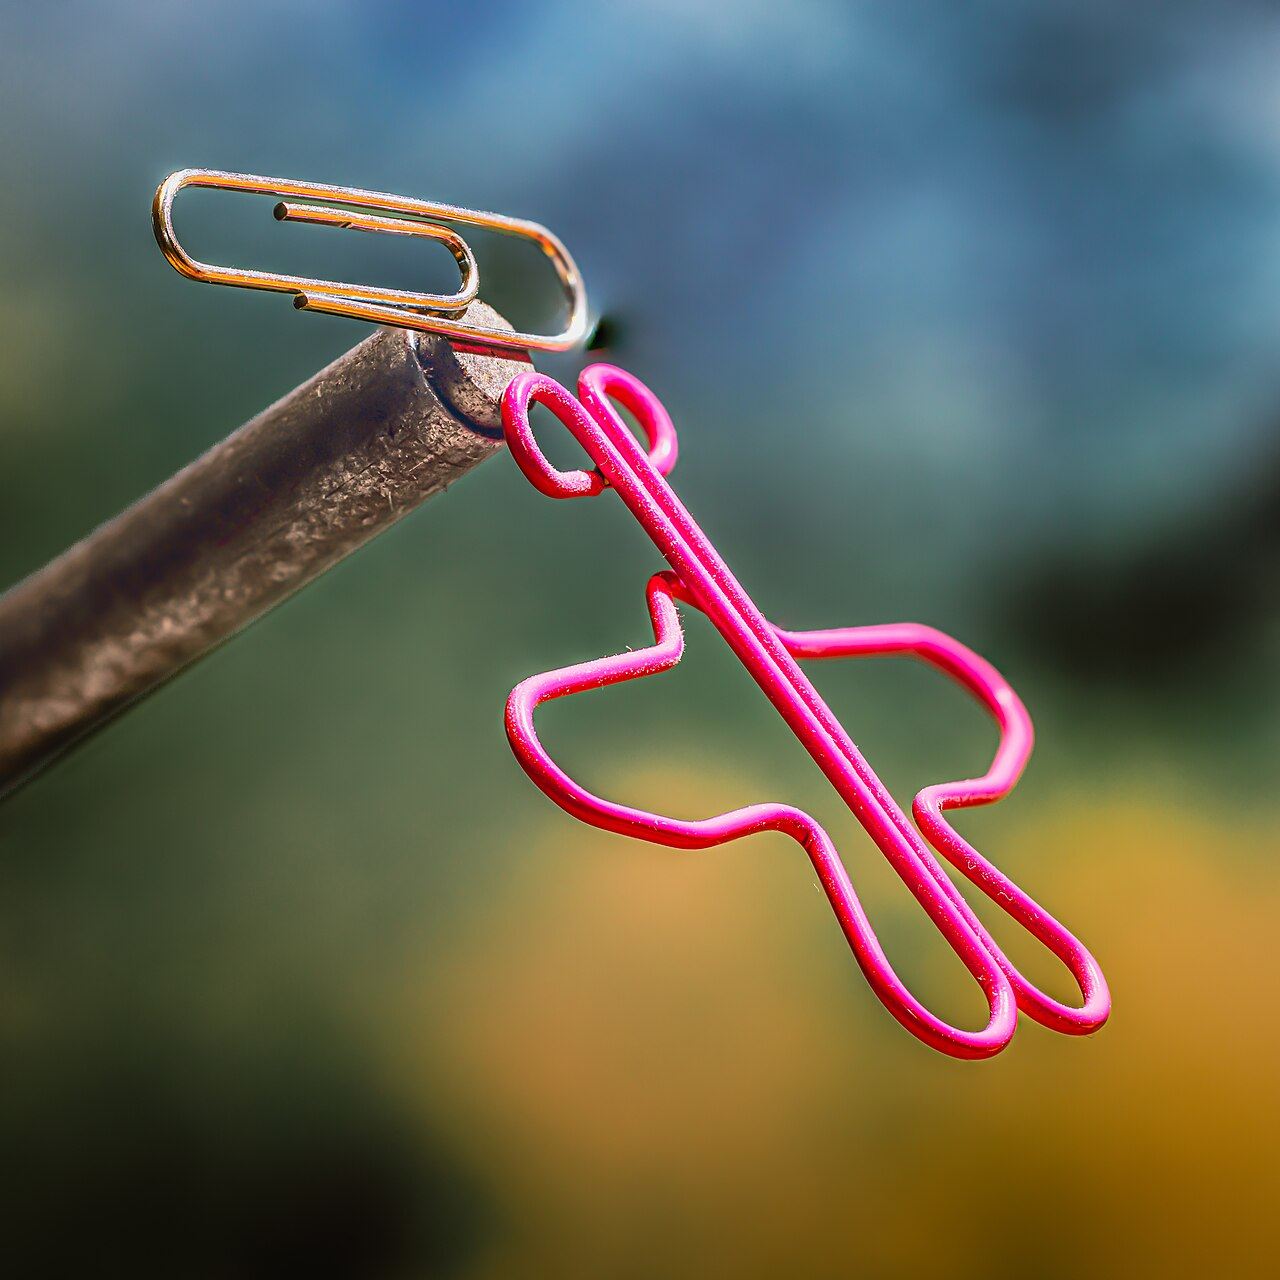
\includegraphics[width=0.5\linewidth]{images/book1/magnet-paperclips.jpg}

{\small Real \omterm{def:g1:magnets:magnet}{magnets} at work: paperclips hang from the tip of a
magnetized rod. The pink clip is coated in plastic --- the pull
passes straight through its coat. \emph{Photo: Donald Olszewski,
CC BY 4.0.}}
\end{omfigure}

\begin{method}[Magnet fishing]\label{met:g1:magnets:fishing}
A game for two, and a fair test of the reach:
\begin{enumerate}
  \item Tie a \omterm{def:g1:magnets:magnet}{magnet} to a string --- this is the fishing rod;
  \item scatter paperclips on the floor --- these are the fish;
  \item lower the \omterm{def:g1:magnets:magnet}{magnet} slowly from high above one clip;
  \item stop lowering the moment the clip jumps up to the \omterm{def:g1:magnets:magnet}{magnet}.
\end{enumerate}
The jump happens only when the \omterm{def:g1:magnets:magnet}{magnet} is close: the pull is strong
near the \omterm{def:g1:magnets:magnet}{magnet} and fades quickly farther away.
\end{method}

\section{Two magnets together}

\begin{example}[Try it: pull or push?]\label{ex:g1:magnets:twomagnets}
Take two \omterm{def:g1:magnets:magnet}{magnets}, one in each hand, and bring their ends slowly
together. Sometimes they leap at each other and snap together.
Now turn one \omterm{def:g1:magnets:magnet}{magnet} around, other end first: bring them together
again, and this time you feel a soft, springy \emph{push} --- the
\omterm{def:g1:magnets:magnet}{magnets} refuse to touch, as if an invisible cushion sat between
them. Same two \omterm{def:g1:magnets:magnet}{magnets}: one way they pull, turned around they push.
\end{example}

\begin{omfigure}
\begin{tikzpicture}[scale=0.85]
  % different colors face each other: attraction
  \draw[thick, fill=red!70] (0,1.1) rectangle (0.9,1.8);
  \draw[thick, fill=blue!60] (0.9,1.1) rectangle (1.8,1.8);
  \draw[thick, fill=red!70] (3.4,1.1) rectangle (4.3,1.8);
  \draw[thick, fill=blue!60] (4.3,1.1) rectangle (5.2,1.8);
  \draw[-Stealth, very thick] (1.95,1.45) -- (2.5,1.45);
  \draw[-Stealth, very thick] (3.25,1.45) -- (2.7,1.45);
  \node[below, font=\small, align=center] at (2.6,0.85)
    {different colors face:\\they leap together};
  % same colors face each other: repulsion
  \draw[thick, fill=red!70] (7.0,1.1) rectangle (7.9,1.8);
  \draw[thick, fill=blue!60] (7.9,1.1) rectangle (8.8,1.8);
  \draw[thick, fill=blue!60] (10.4,1.1) rectangle (11.3,1.8);
  \draw[thick, fill=red!70] (11.3,1.1) rectangle (12.2,1.8);
  \draw[-Stealth, very thick] (6.85,1.45) -- (6.3,1.45);
  \draw[-Stealth, very thick] (12.35,1.45) -- (12.9,1.45);
  \node[below, font=\small, align=center] at (9.6,0.85)
    {same colors face:\\they push apart};
\end{tikzpicture}

{\small Two \omterm{def:g1:magnets:magnet}{magnets} with colored ends, twice. When two
\emph{different} ends face each other, the \omterm{def:g1:magnets:magnet}{magnets} pull together;
flip one so the \emph{same} ends face, and they push each other
away.}
\end{omfigure}

\begin{remark}[The two ends]\label{rem:g1:magnets:ends}
So the two ends of a \omterm{def:g1:magnets:magnet}{magnet} are not the same, even when they look
alike! Each \omterm{def:g1:magnets:magnet}{magnet} has two different ends, and the game of pull and
push depends on \emph{which} ends meet. Try the paperclip test too:
clips cluster at the two ends of a bar \omterm{def:g1:magnets:magnet}{magnet} and mostly ignore its
middle. These two special ends have names and a famous job ---
guiding travelers across the world --- but that story waits for a
later year of this book.
\end{remark}

\section{Exercises}

\begin{exercise}[$\star$]\label{exo:g1:magnets:1}
Sort into ``the \omterm{def:g1:magnets:magnet}{magnet} grabs it'' and ``the \omterm{def:g1:magnets:magnet}{magnet} ignores it'': a
nail; \ a cork; \ a paperclip; \ a plastic duck; \ a steel spoon; \ a
sheet of paper.
\end{exercise}

\begin{exercise}[$\star$]\label{exo:g1:magnets:2}
Which stuff does a \omterm{def:g1:magnets:magnet}{magnet} love? Name two metals or materials the
\omterm{def:g1:magnets:magnet}{magnet} ignores anyway.
\end{exercise}

\begin{exercise}[$\star$]\label{exo:g1:magnets:3}
A drawing holds on the refrigerator door under a \omterm{def:g1:magnets:magnet}{magnet} figure. What
is between the \omterm{def:g1:magnets:magnet}{magnet} and the door? What does this show about the
\omterm{def:g1:magnets:magnet}{magnet}'s pull?
\end{exercise}

\begin{exercise}[$\star$]\label{exo:g1:magnets:4}
A paperclip falls into a glass full of water. How can you get it out
with a \omterm{def:g1:magnets:magnet}{magnet}, without wetting your fingers?
\end{exercise}

\begin{exercise}[$\star$]\label{exo:g1:magnets:5}
In the \omterm{def:g1:magnets:magnet}{magnet} fishing game of \cref{met:g1:magnets:fishing}, the clip
jumps only when the \omterm{def:g1:magnets:magnet}{magnet} comes close. What does this tell you about
the pull far from the \omterm{def:g1:magnets:magnet}{magnet}?
\end{exercise}

\begin{exercise}[$\star$]\label{exo:g1:magnets:6}
Bring two \omterm{def:g1:magnets:magnet}{magnets} end to end: they snap together. What single move
makes the same two \omterm{def:g1:magnets:magnet}{magnets} push apart instead?
\end{exercise}

\begin{exercise}[$\star$]\label{exo:g1:magnets:7}
Where do paperclips cluster on a bar \omterm{def:g1:magnets:magnet}{magnet}: at the middle, or at
the ends? What does this say about where a \omterm{def:g1:magnets:magnet}{magnet} is strongest?
\end{exercise}

\begin{exercise}[$\star$]\label{exo:g1:magnets:8}
Name one way a \omterm{def:g1:magnets:magnet}{magnet} is like your hand moving a toy, and one way it
is completely different. (Think of
\cref{rem:g1:magnets:notouch}.)
\end{exercise}

\begin{exercise}[$\star\star$]\label{exo:g1:magnets:9}
Tom says: ``\omterm{def:g1:magnets:magnet}{Magnets} \omterm{def:g1:magnets:magnet}{attract} everything made of metal.'' Design a
little experiment with a coin, a nail and kitchen foil to test Tom's
sentence, say what will happen --- and correct his sentence.
\end{exercise}
